\exo{12}{Calculer} : Effectuer les calculs suivants en détaillant les étapes.

\begin{multicols}{4}
    $$\dfrac{4}{7}+\dfrac{5}{7}$$ \vspace*{2.5cm}\columnbreak

    $$\dfrac{2}{4}+\dfrac{5}{3}$$ \vspace*{2.5cm}\columnbreak

    $$\dfrac{5}{8}-\dfrac{3}{8}$$ \vspace*{2.5cm}\columnbreak

    $$\dfrac{2}{5}-\dfrac{3}{7}$$ \vspace*{2.5cm}
\end{multicols}

\begin{multicols}{4}
    $$\dfrac{3}{4}\times\dfrac{9}{5}$$ \vspace*{2.5cm}\columnbreak

    $$\dfrac{3}{7}\times\dfrac{5}{6}$$ \vspace*{2.5cm}\columnbreak

    $$\dfrac{2}{9}\div\dfrac{4}{3}$$ \vspace*{2.5cm}\columnbreak

    $$\dfrac{3}{8}\div\dfrac{5}{7}$$ \vspace*{2.5cm}
\end{multicols}

\begin{multicols}{2}
    $$-17-3\times (-2)+8$$ \vspace*{4cm}\columnbreak

    $$(-3)\times 6 \div 2\times 3-1$$ \vspace*{4cm}
\end{multicols}

\begin{multicols}{2}
    $$(-5\times 5 -2+5)\div (-2)-9$$ \vspace*{4cm}\columnbreak

    $$-2\times (3+3\times 3 -3\div 3)$$ \vspace*{4cm}
\end{multicols}

\exo{4}{Raisonner} : Calculer le volume des deux solides suivants.

\begin{minipage}[t]{0.45\textwidth}
    \begin{figure}[H]
        \centering
        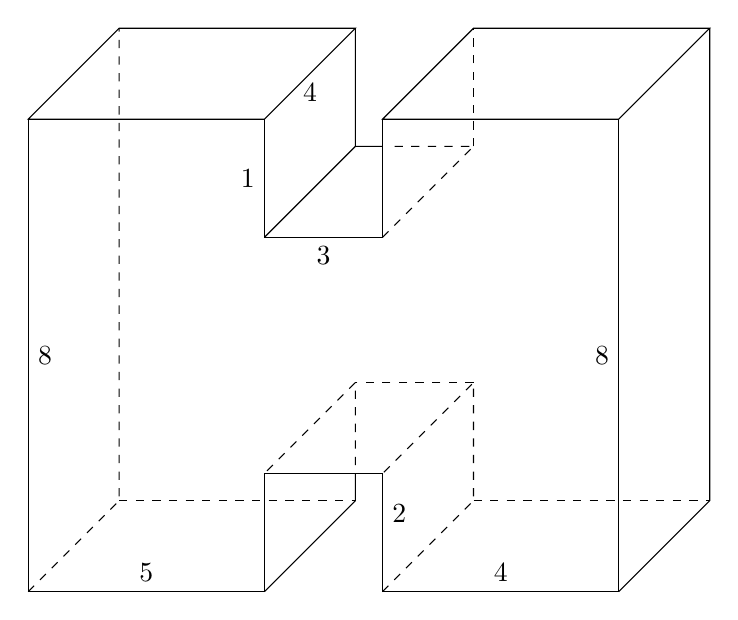
\begin{tikzpicture}[scale=1.5]
            \draw (0,4,0) --(2,4,0) -- node [midway,below] {4}  (2,4,-2) -- (0,4,-2)--cycle; %Face haute gauche
            \draw (3,4,0) --(5,4,0) -- (5,4,-2) -- (3,4,-2)--cycle; %Face haute droite
            \draw (5,0,0) -- (5,0,-2) -- (5,4,-2); %Cote droit
            \draw (2,0,0) -- (2,0,-2) -- (2,4,-2); %A faire en cavaliere
            \draw [fill=white] (2,3,0) --(2,3,-2) -- (3,3,-2)--(3,3,0); %Millieu haut
            \draw [fill=white] (0,0,0) --node [midway,above] {5} (2,0,0)-- (2,1,0)-- (3,1,0)-- node [midway,above right] {2} (3,0,0)--node [midway,above] {4} (5,0,0)--node [midway,left] {8}(5,4,0)--(3,4,0)-- (3,3,0)--node [midway,below] {3}(2,3,0) --node [midway,left] {1}(2,4,0)-- (0,4,0)--node[midway,right]{8} cycle; %Face avant
            \draw[dashed] (3,0,-2) --(5,0,-2);
            \draw[dashed] (3,0,0)--(3,0,-2)--(3,1,-2)--(3,1,0);
            \draw[dashed] (3,1,-2)--(2,1,-2);
            \draw[dashed] (0,0,-2) --(2,0,-2);
            \draw[dashed] (0,0,0)--(0,0,-2)--(0,4,-2);
            \draw[dashed] (2,0.3,-2)--(2,1,-2)--(2,1,0);
            \draw[dashed] (3,3,0)--(3,3,-2)--(2.3,3,-2);
            \draw[dashed] (3,3,-2)--(3,4,-2);
        \end{tikzpicture}
    \end{figure}
\end{minipage}
\hfill
\vrule
\hfill
\begin{minipage}[t]{0.45\textwidth}
    \begin{figure}[H]
        \centering
        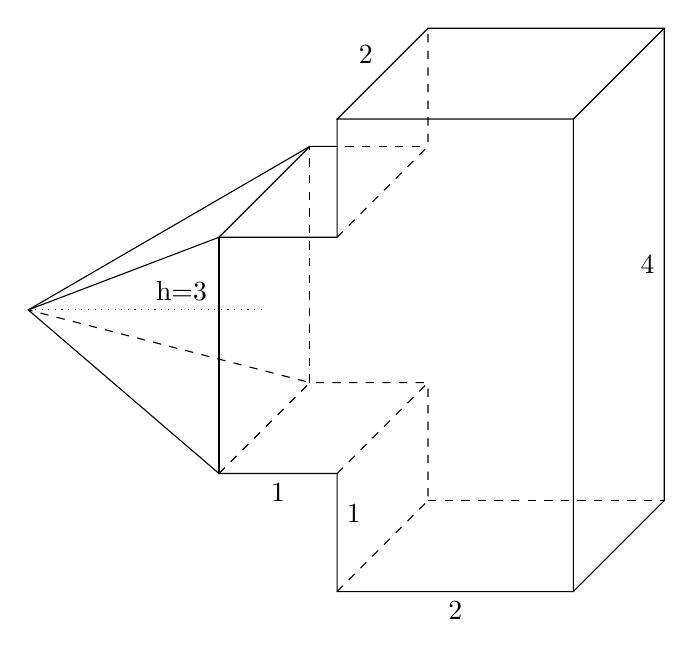
\begin{tikzpicture}[scale=1.5]
            \draw (3,4,0) --(5,4,0) -- (5,4,-2) -- (3,4,-2)-- node[midway,above left]{2} cycle; %Face haute droite
            \draw (5,0,0) -- (5,0,-2) -- node [midway,left] {4}(5,4,-2); %Cote droit
            \draw [fill=white] (2,3,0) --(2,3,-2) -- (3,3,-2)--(3,3,0); %Millieu haut
            \draw (2,3,-2)--(0,2,-1);
            \draw[fill=white] (0,2,-1)--(2,1,0)--node [midway,below] {1} (3,1,0)--node [midway,above right] {1} (3,0,0)--node [midway,below] {2} (5,0,0)--(5,4,0)--(3,4,0)--(3,3,0)--(2,3,0)--cycle; %Face avant
            \draw[dashed] (2,1,0)-- (2,1,-2)--(0,2,-1);
            \draw[dashed] (2,1,-2)--(2,3,-2);
            \draw (2,1,0)--(2,3,0);
            \draw[dashed] (3,0,-2) --(5,0,-2);
            \draw[dashed] (3,0,0)--(3,0,-2)--(3,1,-2);
            \draw[dotted] (0,2,-1)-- node [midway,above right]{h=3}(2,2,-1);
            \draw[dashed] (3,1,0)--(3,1,-2)--(2,1,-2);
            \draw[dashed] (3,3,0)--(3,3,-2)--(3,4,-2);
            \draw[dashed] (2.3,3,-2)--(3,3,-2);
        \end{tikzpicture}
    \end{figure}
    \vspace{17em}
\end{minipage}

\exo{4}{Chercher} :

Pour les besoins d'une vidéo, Squeezie cherche à remplir une piscine de béton. 
La piscine est un cylindre de rayon 1~m et de hauteur 0,8~m. 
1~L de béton est composé de $\dfrac{1}{4}$ d'eau, $\dfrac{1}{4}$ de ciment et $\dfrac{1}{2}$ de sable.

En considérant que l'eau coûte 0,04~€/L ; le sable 2~€/L et le ciment 0,2~€/L combien va lui coûter cette expérience ?
